% !TeX TXS-program:compile = txs:///arara
% arara: pdflatex: {shell: yes, synctex: no, interaction: batchmode}
% arara: pdflatex: {shell: yes, synctex: no, interaction: batchmode} if found('log', '(undefined references|Please rerun|Rerun to get)')

\documentclass[a4paper]{article}
\usepackage[french]{babel}
\usepackage[utf8]{inputenc}
\usepackage[T1]{fontenc}
\usepackage{PapierGurvan}
\usepackage{amsmath,amssymb}
\usepackage{fontawesome5}
\usepackage{enumitem}
\usepackage{tabularray}
\usepackage{fancyvrb}
\usepackage{fancyhdr}
\usepackage{frcursive}
\usepackage{aurical}
\fancyhf{}
\renewcommand{\headrulewidth}{0pt}
\lfoot{\sffamily\small [PapierGurvan]}
\cfoot{\sffamily\small - \thepage{} -}
\rfoot{\hyperlink{matoc}{\small\faArrowAltCircleUp[regular]}}

%\usepackage{hvlogos}
\usepackage{hologo}
\providecommand\tikzlogo{Ti\textit{k}Z}
\providecommand\TeXLive{\TeX{}Live\xspace}
\providecommand\PSTricks{\textsf{PSTricks}\xspace}
\let\pstricks\PSTricks
\let\TikZ\tikzlogo
\newcommand\TableauDocumentation{%
	\begin{tblr}{width=\linewidth,colspec={X[c]X[c]X[c]X[c]X[c]X[c]},cells={font=\sffamily}}
		{\huge \LaTeX} & & & & &\\
		& {\huge \hologo{pdfLaTeX}} & & & & \\
		& & {\huge \hologo{LuaLaTeX}} & & & \\
		& & & {\huge \TikZ} & & \\
		& & & & {\huge \TeXLive} & \\
		& & & & & {\huge \hologo{MiKTeX}} \\
	\end{tblr}
}

\usepackage{hyperref}
\urlstyle{same}
\hypersetup{pdfborder=0 0 0}
\usepackage[margin=1.5cm]{geometry}
\setlength{\parindent}{0pt}
\definecolor{LightGray}{gray}{0.9}

\def\TPversion{0.1.0}
\def\TPdate{11 septembre 2023}

\usepackage[most]{tcolorbox}
\tcbuselibrary{minted}
\NewTCBListing{PresentationCode}{ O{blue} m }{%
	sharp corners=downhill,enhanced,arc=12pt,skin=bicolor,%
	colback=#1!1!white,colframe=#1!75!black,colbacklower=white,%
	attach boxed title to top right={yshift=-\tcboxedtitleheight},title=Code \LaTeX,%
	boxed title style={%
		colframe=#1!75!black,colback=#1!15!white,%
		,sharp corners=downhill,arc=12pt,%
	},%
	fonttitle=\color{#1!90!black}\itshape\ttfamily\footnotesize,%
	listing engine=minted,minted style=colorful,
	minted language=tex,minted options={tabsize=4,fontsize=\footnotesize,autogobble},
	#2
}

\newcommand\Cle[1]{{\bfseries\sffamily\textlangle #1\textrangle}}

\begin{document}

\pagestyle{fancy}

\thispagestyle{empty}

\vspace{2cm}

\begin{center}
	\begin{minipage}{0.75\linewidth}
	\begin{tcolorbox}[colframe=yellow,colback=yellow!15]
		\begin{center}
			\begin{tabular}{c}
				{\Huge \texttt{PapierGurvan [fr]}}\\
				\\
				{\LARGE Pour créer et écrire sur les} \\
				\\
				{\LARGE lignes d'un papier Gurvan.}
			\end{tabular}
			
			\medskip
			
			{\small \texttt{Version \TPversion{} -- \TPdate}}
		\end{center}
	\end{tcolorbox}
\end{minipage}
\end{center}

\vspace{0.5cm}

\begin{center}
	\begin{tabular}{c}
	\texttt{Cédric Pierquet}\\
	{\ttfamily c pierquet -- at -- outlook . fr}\\
	\texttt{\url{https://github.com/cpierquet/PapierGurvan}}
\end{tabular}
\end{center}

\vspace{0.5cm}

{$\blacktriangleright$~~Créer une grille type papier Gurvan (créé par Anne-Gaël Tissot), et éventuellement écrire sur les lignes.}

\smallskip

{$\blacktriangleright$~~Créer une feuille complète type papier Gurvan, et éventuellement écrire sur les lignes.}

\vspace{1cm}

\begin{center}
\begin{EnvGurvan}[NbCarreaux=17x5,Interligne=2.5]
	\EcrireLigneGurvan[Echelle=1.925]{\cursive une petite ligne\ldots}
	\EcrireLigneGurvan[Echelle=1.925]{\cursive une autre petite ligne\ldots}
	\EcrireLigneGurvan[Echelle=2.125]{\Fontskrivan encore une autre ligne\ldots}
	\EcrireLigneGurvan[Echelle=2.125]{\Fontskrivan une dernière petite ligne\ldots}
\end{EnvGurvan}
\end{center}

\vspace{0.5cm}

\hfill{}\textit{Merci à Laurent LC pour son idée et ses retours.}

\vfill

\hrule

\medskip

\TableauDocumentation

\medskip

\hrule

\medskip

\newpage

\phantomsection
\hypertarget{matoc}{}

\tableofcontents

\newpage

\section{Le package PapierGurvan}

\subsection{Chargement du package, packages utilisés}

Le package \textsf{PapierGurvan} se charge dans le préambule via la commande :

\begin{PresentationCode}{listing only}
\usepackage{PapierGurvan}
\end{PresentationCode}

Il est compatible avec les compilations usuelles en \textsf{latex}, \textsf{pdflatex}, \textsf{lualatex} ou \textsf{xelatex}.

\medskip

Pour des soucis de compatibilité, \texttt{xcolor} n'est pas chargé avec des options spécifiques, les couleurs utiles ont été définies directement dans le package.

\medskip

Il charge les packages et librairies suivantes :

\begin{itemize}
	\item \texttt{tikz} avec les librairies \Cle{calc} et \Cle{positionning} ;
	\item \texttt{xstring}, \texttt{simplekv} et \texttt{setspace}.
\end{itemize}

\subsection{\og Philosophie \fg{} du package}

L'idée est de proposer, comme pour le package \texttt{WriteOngrid}, des \textsf{commandes} et \textsf{environnements} pour travailler sur un quadrillage de type Gurvan et écrire \og sur les lignes \fg.

\smallskip

J'ai choisi de ne pas intégrer les commandes et environnements suivants dans le package \texttt{WriteOnGrid} car la portée de celles-ci est différente, du fait de la spécificité du papier Gurvan.

\medskip

L'auteure, Anne-Gaël Tissot, sur le site \href{http://www.sos-ecriture.fr/2012/09/lignages-decriture-agrandis.html}{sos-ecriture.fr} présente le papier Gurvan :

\medskip

\begin{tblr}{width=\linewidth,colspec={Q[m,c,2cm]|[1pt]X[m,j]},cells={font=\small\sffamily}}
	\scalebox{3}[3]{\faBookReader} & {En rééducation, j'utilise parfois des lignes d'écriture basées sur du Seyès, mais modifiées afin d'aider les enfants en difficulté. La ligne de base est nettement différenciée. La zone médiane (dans laquelle s'écrivent les lettres a, c, e, i, m, n, o, r, s, u, v et w) est en couleur foncée, les zones haute et basse en couleur plus claire. \\ Les lignes de base sont également plus écartées que dans les cahiers classiques, afin que les lettres basses (comme le f) ne chevauchent pas les lettres hautes (comme le l) écrites à la ligne du dessous. \\
	À gauche, se trouve une marge notée par un trait rouge. À droite, une seconde marge pointillée, pour aider les enfants à aller à la ligne au bon moment. [...] Si le lignage habituel est trop petit pour des élèves de maternelle ou début CP, les lignages les plus grands ne sont pas forcément les plus adaptés pour les enfants, qui ont de petites mains et dont les doigts auront parfois du mal à faire de grandes lettres. Je teste toujours, pour chaque enfant, l'espacement des lignes d'écriture qui convient le mieux.} \\
\end{tblr}

\medskip

L'idée serait donc d'utiliser une telle \textit{grille} avec une police type \og calligraphie \fg, comme la police \texttt{frcursive} disponible en natif dans les distributions \LaTeX.

\medskip

D'autres exemples sont fournis en marge de cette documentation, qui montrent l'utilisation de \texttt{PapierGurvan} avec une police (non présente en natif) \texttt{BelleAllure} qui peut-être utilisée avec une compilation en \hologo{LuaLaTeX}.

\hfill~\href{https://www.dafont.com/fr/belle-allure.font}{[source]}

\begin{center}
	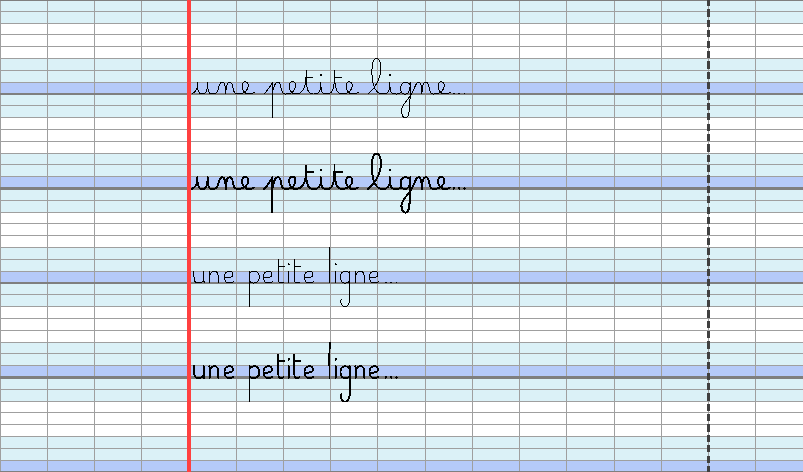
\includegraphics{BelleAllure.pdf}
\end{center}

%\subsection{Fonctionnement global}
%
%La grille est créée en spécifiant le nombre de carreaux (sous la forme nbCol$\times$nbLig), et on peut ensuite spécifier des \textit{débordements} latéraux pour éventuellement étendre le quadrillage dans les marges (gauche et droite). On peut également \textit{jouer} sur la marge, pour commencer les lignes à un niveau donné.
%
%\medskip
%
%Ci-dessous on représente une grille $5\times5$ :
%
%\begin{itemize}
%	\item de taille 24x5 ;
%	\item avec un élargissement de \textcolor{red}{2 carreaux à gauche} et \textcolor{blue}{3 carreaux à droite} ;
%	\item en commençant à écrire au niveau du \textcolor{orange}{1\up{er} carreau} ;
%	\item un \textcolor{green!50!black}{\textit{cadre}} est rajouté pour visualiser la grille \textit{de base}.
%\end{itemize}
%
%\medskip
%
%\begin{tikzpicture}
%	\useasboundingbox (0,0) rectangle ({0.5*24},{-0.5*5}) ;
%	\draw[xstep=0.5,ystep=0.5,thin,lightgray!50] ({-0.5*2},0) grid ({0.5*24+0.5*3},{-0.5*5}) ;
%	\draw[thick,decorate,decoration={brace,amplitude=8pt,mirror}](0,{-0.5*5-0.25})--({0.5*24},{-0.5*5-0.25}) node[midway,below=8pt,font=\small\sffamily] {24C} ;
%	\draw[red,thick,decorate,decoration={brace,amplitude=8pt,mirror}] ({-2*0.5},{-0.5*5-0.25})--({0},{-0.5*5-0.25}) node[midway,below=8pt,font=\small\sffamily] {2C} ;
%	\draw[blue,thick,decorate,decoration={brace,amplitude=8pt,mirror}] ({0.5*24},{-0.5*5-0.25})--({0.5*24+3*0.5},{-0.5*5-0.25}) node[midway,below=8pt,font=\small\sffamily] {3C} ;
%	\draw[thick,decorate,decoration={brace,amplitude=8pt}] ({0.5*24+3*0.5+0.25},0)--({0.5*24+3*0.5+0.25},{-0.5*5}) node[midway,right=8pt,font=\small\sffamily] {5C} ;
%	\draw[very thick,orange,densely dashed] ({0.5*1},0)--({0.5*1},{-0.5*5}) ;
%	\draw[green!50!black,thick] (0,0) rectangle ({0.5*24},{-0.5*5}) ;
%\end{tikzpicture}
%
%\vspace{1.5cm}
%
%Il est à noter que le figure \texttt{tikzpicture} est \textit{délimitée} par le \textcolor{green!50!black}{\textit{cadre}}, afin de pouvoir gérer les débordements et l'alignement de l'environnement !
%
%\smallskip
%
%De plus, le bord gauche du \textcolor{green!50!black}{\textit{cadre}} est aligné sur la marge gauche de la page, donc la position du quadrillage dépend en partie de la configuration de \texttt{\textbackslash parindent}.
%
%\pagebreak
%

\pagebreak

\subsection{Couleurs prédéfinies}

Le package \textsf{PapierGurvan} définit également des couleurs pour une saisie plus facile !

\begin{PresentationCode}{listing only}
\definecolor{GurvanBleuFonce}{HTML}{B5CAF9}
\definecolor{GurvanBleuCiel}{HTML}{DBF1F7}
\def\ColGgurvan{gray!75/GurvanBleuFonce/GurvanBleuCiel}%réglure+fondfonce+fondclair
\end{PresentationCode}

\section{Grilles individuelles}

\subsection{La commande}

\begin{PresentationCode}{listing only}
%commande francisée, avec clés en français pour préparer la grille

\PapierGurvan[clés]<couleur(s)>
\end{PresentationCode}

Le premier argument, \textit{optionnel}, entre \texttt{[...]} propose les \Cle{clés} :

\begin{itemize}
	\item \Cle{NbCarreaux} pour spécifier le nombre de carreaux, sous la forme \texttt{(nbCol)x(nbLig)} ; \hfill~défaut : \Cle{17x5}
	\item \Cle{Unite} pour spécifier l'échelle de la figure ; \hfill~défaut : \Cle{1}
	\item \Cle{Marge} pour spécifier la \textcolor{orange}{marge} du début des lignes ; \hfill~défaut : \Cle{4}
	\item le booléen \Cle{AffBarres} pour afficher ou non la marge ; \hfill~défaut : \Cle{true}
%	\item \Cle{Elargir} pour préciser les carreaux de débordements, sous la forme unique \texttt{\textcolor{red}{G}\textcolor{blue}{D}} ou par côté \texttt{\textcolor{red}{G}/\textcolor{blue}{D}} ;\hfill~défaut : \Cle{0}
%	\item le booléen \Cle{Cadre} pour afficher le cadre de base du quadrillage ;\hfill~défaut : \Cle{false}
%	\item la clé \Cle{Grille}, parmi \Cle{5x5 / Seyes / Ruled}, pour spécifier le type de quadrillage ;\hfill~défaut : \Cle{5x5}
	\item la clé \Cle{Interligne} pour sprécifier (ne mm) l'interligne voulu ; \hfill~défaut : \Cle{3}
	\item la clé \Cle{CouleurBarre} pour la barre de marge .\hfill~défaut : \Cle{red!75}
\end{itemize}

Le second argument, \textit{optionnel}, entre \texttt{<...>} correspond quant à lui aux couleurs de base du quadrillage :

\begin{itemize}
	\item sous la forme \Cle{CouleurR/CouleurF/CouleurC} (\Cle{gray!75/GurvanBleuFonce/GurvanBleuCiel} pour la réglure, le fond foncé et le fond clair ;
	\item sous la forme \Cle{Couleur} pour une base monochrome.
\end{itemize}

\begin{PresentationCode}{}
\PapierGurvan[Interligne=3,NbCarreaux=10x2,Marge=2]
\end{PresentationCode}

\begin{PresentationCode}{}
\PapierGurvan[Interligne=2,NbCarreaux=14x3,Marge=1]<lightgray>
\end{PresentationCode}

\subsection{L'environnement}

\begin{PresentationCode}{listing only}
%environnement francisé, avec clés en français pour préparer la grille

\begin{EnvGurvan}[clés]<couleur(s)>
	%commandes
\end{EnvGurvan}
\end{PresentationCode}

Le premier argument, \textit{optionnel}, entre \texttt{[...]} propose les \Cle{clés} :

\begin{itemize}
	\item \Cle{NbCarreaux} pour spécifier le nombre de carreaux, sous la forme \texttt{(nbCol)x(nbLig)} ; \hfill~défaut : \Cle{17x5}
	\item \Cle{Unite} pour spécifier l'échelle de la figure ; \hfill~défaut : \Cle{1}
	\item \Cle{Marge} pour spécifier la \textcolor{orange}{marge} du début des lignes ; \hfill~défaut : \Cle{4}
	\item le booléen \Cle{AffBarres} pour afficher ou non la marge ; \hfill~défaut : \Cle{true}
	%	\item \Cle{Elargir} pour préciser les carreaux de débordements, sous la forme unique \texttt{\textcolor{red}{G}\textcolor{blue}{D}} ou par côté \texttt{\textcolor{red}{G}/\textcolor{blue}{D}} ;\hfill~défaut : \Cle{0}
	%	\item le booléen \Cle{Cadre} pour afficher le cadre de base du quadrillage ;\hfill~défaut : \Cle{false}
	%	\item la clé \Cle{Grille}, parmi \Cle{5x5 / Seyes / Ruled}, pour spécifier le type de quadrillage ;\hfill~défaut : \Cle{5x5}
	\item la clé \Cle{Interligne} pour sprécifier (en mm) l'interligne voulu ; \hfill~défaut : \Cle{3}
	\item la clé \Cle{CouleurBarre} pour la barre de marge .\hfill~défaut : \Cle{red!75}
\end{itemize}

Le second argument, \textit{optionnel}, entre \texttt{<...>} correspond quant à lui aux couleurs de base du quadrillage :

\begin{itemize}
	\item sous la forme \Cle{CouleurR/CouleurF/CouleurC} (\Cle{gray!75/GurvanBleuFonce/GurvanBleuCiel} pour la réglure, le fond foncé et le fond clair ;
	\item sous la forme \Cle{Couleur} pour une base monochrome.
\end{itemize}

\medskip

\begin{PresentationCode}{}
\begin{EnvGurvan}
\end{EnvGurvan}
\end{PresentationCode}

\begin{PresentationCode}{}
\begin{EnvGurvan}[NbCarreaux=14x3,Interligne=2,Marge=2]
\end{EnvGurvan}
\end{PresentationCode}

\subsection{Écrire sur les lignes}

L'idée est maintenant de pouvoir écrire sur les lignes du quadrillage créé (environnement !), et pour garantir le fait d'écrire \textit{pile} sur la ligne, on applique les recommandations suivantes :

\begin{itemize}
	\item les lignes doivent être saisies une par une, du \og haut \fg{} vers le \og bas \fg{} ;
	\item pas de paragraphe \textit{multilignes}, pas de puce ou de numérotation ;
	\item une ligne peut être passée.
\end{itemize}

\begin{PresentationCode}{listing only}
...
	%pour saisir les lignes, une par une
	\EcrireLigneGurvan[clés]<alignement>{texte}
	%pour passer la ligne
	\PasseLigneGurvan
...
\end{PresentationCode}

Le premier argument, entre \texttt{[...]} propose les \Cle{clés} :

\begin{itemize}
	\item \Cle{DecalH} pour spécifier le décalage horizontal (en carreaux) de la ligne, par rapport à la \textcolor{orange}{marge} ; \hfill~défaut : \Cle{0}
	\item \Cle{DecalV} pour spécifier le décalage vertical du texte par rapport à la ligne ; \hfill~défaut : \Cle{0pt}
	\item \Cle{Echelle} pour spécifier l'échelle du texte à écrire.\hfill~défaut : \Cle{1}
\end{itemize}

Le deuxième argument, \textit{optionnel}, entre \texttt{<...>} permet de spécifier l'alignement horizontal entre les \textit{marges} (parmi \Cle{left/center/right}) du texte (\Cle{left} par défaut).

\medskip

Le troisième argument, \textit{obligatoire} et entre \texttt{\{...\}} est quant à lui le texte à saisir, avec possibilité de spécifier taille, couleur, fonte, etc

\begin{PresentationCode}{}
\begin{EnvGurvan}[Marge=1,Interligne=2,NbCarreaux=17x4]
	\EcrireLigneGurvan{mon texte sur la ligne 1\ldots}
	\EcrireLigneGurvan[Echelle=1.25]<center>{\ttfamily mon texte, en fonte teletype +25\,\%, centré sur la ligne 2\ldots}
	\PasseLigneGurvan{\sffamily mon texte, en fonte sans réduite de 50\,\%, sur la ligne 4\ldots}
	\EcrireLigneGurvan[DecalH=1.5]{\cursive mon texte sur la ligne 7, décalé de 1.5 carreaux\ldots}
\end{EnvGurvan}
\end{PresentationCode}
\pagebreak

\section{Page complète type Gurvan}

\subsection{Idée et fonctionnement global}

Il s'agit ici de créer le quadrillage Gurvan sur la page complète, comme pour la copie d'un élève !

\smallskip

\faBomb{} Le fonctionnement est différent des environnements \textit{ponctuels} précédents, et l'écriture sur les lignes du quadrillage peuvent poser souci avec des environnements mathématiques !!

\medskip

La grille complète est liée à un environnement (basé sur \texttt{tikzpicture}), et les commandes pour écrire sont à mettre dans l'environnement.

\smallskip

Tout le placement est géré grâce à un point (fictif), nommé \texttt{(GurvanOrigine)}, qui correspond au point de départ de l'écriture sur la copie !
%
\begin{PresentationCode}{listing only}
\begin{PleinePageGurvan}[options]
	\LigneGurvan[options]<alignement>(ajustement){texte}
	\ParagrapheGurvan[options]<alignement>(ajustement){texte}
\end{PleinePageGurvan}
\end{PresentationCode}

\subsection{La grille}

Pour l'environnement de création de la grille, l'argument, \textit{optionnel} et entre \texttt{[...]}, propose :

\begin{itemize}
	\item la clé \Cle{Interligne} pour spécifier (en mm) l'interligne voulu ; \hfill~défaut : \Cle{3}
	\item la clé \Cle{Papier}, \Cle{A4 ou A5}, pour spécifier le format ; \hfill~défaut : \Cle{A4}
	\item la clé \Cle{Marges}, sous la forme \Cle{MargeGauche/MargeDroite} pour la position (en carreaux) des deux marges verticales ; \hfill~défaut : \Cle{5/2}
	\item la clé \Cle{CoulLignes} pour la couleur des \textit{réglures} ;\hfill~défaut : \Cle{gray!75}
	\item la clé \Cle{CoulFondClair} pour la couleur de fond \textit{clair} ;\hfill~défaut : \Cle{GurvanBleuCiel}
	\item la clé \Cle{CoulFondFonce} pour la couleur de fond \textit{foncé} ;\hfill~défaut : \Cle{GurvanBleuFonce}
	
	\item le booléen \Cle{NumLignes} pour afficher le numéro des lignes (pour aider !). \hfill~défaut : \Cle{false}
\end{itemize}

\subsection{La commande pour saisir une ligne}

La commande \texttt{LigneGurvan} permet de saisir une ligne \textbf{unique}, un peu comme la commande pour les petits blocs de quadrillage. Plusieurs options et arguments sont disponibles.

\begin{PresentationCode}{listing only}
\LigneGurvan[options]<alignement>(ajustement){texte}
\end{PresentationCode}

La commande positionne le \textsf{texte}, au niveau de la marge verticale, sur la ligne précisée !

\smallskip

Le premier argument, \textit{optionnel} et entre \texttt{[...]} propose :

\begin{itemize}
	\item la clé \Cle{Couleur} pour spécifier une couleur globale pour le texte ;\hfill~défaut : \Cle{black}
	\item la clé \Cle{Echelle} pour spécifier une échelle globale pour le texte ;\hfill~défaut : \Cle{1}
	\item la clé \Cle{Ligne} pour spécifier le numéro de ligne sur lequel on souhaite écrire ;\hfill~défaut : \Cle{1}
	\item la clé \Cle{DecalBord} pour spécifier le décalage (en mm) de la boîte dans laquelle le texte sera placé par rapport aux marges verticales.\hfill~défaut : \Cle{0}
\end{itemize}

Le deuxième argument, \textit{optionnel} et entre \texttt{<...>}, permet de spécifier l'alignement souhaité pour la ligne, parmi \Cle{left/center/right}, et vaut \Cle{left} par défaut.

\smallskip

Le troisième argument, \textit{optionnel} et entre \texttt{(...)}, permet de positionner le texte avec un \textit{décalage fin} et \textit{relatif} de $(x\,;y)$, et il est fixé par défaut à \Cle{0,0}.

\smallskip

Le dernier argument, \textit{obligatoire} et entre \texttt{\{...\}} est le texte à placer, avec les options classiques en langage \TeX{} !

\pagebreak

\subsection{Une commande pour saisir un paragraphe (attention au choix de la police !)}

La commande \texttt{ParagrapheGurvan} permet de saisir des commandes \textit{multilignes}, grâce à l'utilisation de \texttt{\textbackslash\textbackslash}.

\begin{PresentationCode}{listing only}
\ParagrapheGurvan[options]<alignement>(ajustement){texte}
\end{PresentationCode}

\faBomb{} Cet aspect \textit{multilignes} pourra sans doute être problématique pour un placement optimal, donc doit être utilisé avec précautions\ldots

\smallskip

Le premier argument, \textit{optionnel} et entre \texttt{[...]} propose :

\begin{itemize}
	\item la clé \Cle{Ligne} pour spécifier le numéro de ligne sur lequel on souhaite écrire ;\hfill~défaut : \Cle{1}
	\item la clé \Cle{Couleur} pour spécifier une couleur globale pour le texte ;\hfill~défaut : \Cle{black}
	\item la clé \Cle{TaillePolice} pour spécifier la taille, en points, du texte ;\hfill~défaut : \Cle{1}
	\item la clé \Cle{Espacement}, en unité absolue ou \Cle{auto}, pour que l'interligne soit OK ;\hfill~défaut : \Cle{auto}
	\item la clé \Cle{DecalBord} pour spécifier le décalage (en mm) de la boîte dans laquelle le texte sera placé par rapport aux marges verticales.\hfill~défaut : \Cle{0}
\end{itemize}

Le deuxième argument, \textit{optionnel} et entre \texttt{<...>}, permet de spécifier l'alignement souhaité pour la ligne, parmi \Cle{left/center/right/justify}, et vaut \Cle{justify} par défaut.

\smallskip

Le troisième argument, \textit{optionnel} et entre \texttt{(...)}, permet de positionner le paragraphe avec un \textit{décalage fin} et \textit{relatif} de $(x\,;y)$, et il est fixé par défaut à \Cle{0,0}.

\smallskip

Le dernier argument, \textit{obligatoire} et entre \texttt{\{...\}} est le paragraphe à placer, avec les options classiques en langage \TeX{}, et le passage à la ligne effectué par \texttt{\textbackslash\textbackslash} !

\medskip

\faBomb{} À noter que, pour \textit{coller} au lignes horizontales, c'est le paramètre \Cle{Echelle} qui sera à adapter, et il faudra sans doute faire des essais en fonction de la police et de l'interligne !

\subsection{Exemple \og détaillé \fg}

Un exemple \textit{détaillé}, avec le rendu en page suivante, avec quelques commentaires pour expliquer.

\begin{PresentationCode}{listing only}
\pagestyle{empty}

\begin{PleinePageGurvan}[NumLignes]
	%on montre la position du nœud (GurvanOrigine)
	\filldraw[teal] (GurvanOrigine) circle[radius=4pt] ;
	%un texte monoligne avec test pour l'échelle
	\LigneGurvan[Echelle=1.925,DecalBord=8]{\cursive un petit Titre\ldots}
	%un paragraphe complet avec test pour l'échelle
	\ParagrapheGurvan[Ligne=3,Echelle=2.125]{\Fontskrivan On peut essayer avec une dictée, rien de bien méchant.\\
	Il était une fois une petite princesse nommée Pauline, et un gentil dragon nommé Antoine.}
	\ParagrapheGurvan[Ligne=10,Echelle=2.125,DecalBord=4]{\Fontskrivan On peut essayer avec une dictée, rien de bien méchant.\\
	Il était une fois une petite princesse nommée Pauline, et un gentil dragon nommé Antoine.}
\end{PleinePageGurvan}
\end{PresentationCode}

\pagebreak

\pagestyle{empty}

\begin{PleinePageGurvan}[NumLignes]
	%on montre la position du nœud (GurvanOrigine)
	\filldraw[teal] (GurvanOrigine) circle[radius=4pt] ;
	%un texte monoligne avec test pour l'échelle
	\LigneGurvan[Echelle=1.925,DecalBord=8]{\cursive un petit Titre\ldots}
	%un paragraphe complet avec test pour l'échelle
	\ParagrapheGurvan[Ligne=3,Echelle=2.125]{\Fontskrivan On peut essayer avec une dictée, rien de bien méchant.\\
		Il était une fois une petite princesse nommée Pauline, et un gentil dragon nommé Antoine.}
	\ParagrapheGurvan[Ligne=10,Echelle=2.125,DecalBord=4]{\Fontskrivan On peut essayer avec une dictée, rien de bien méchant.\\
		Il était une fois une petite princesse nommée Pauline, et un gentil dragon nommé Antoine.}
\end{PleinePageGurvan}

\pagebreak

\section{Historique}

\verb|v0.1.0|~:~~~~Version initiale

\end{document}